\documentclass[journal,12pt,twocolumn]{IEEEtran}

\usepackage{setspace}
\usepackage{gensymb}

\singlespacing


\usepackage[cmex10]{amsmath}
\usepackage{amsthm}

\usepackage{mathrsfs}
\usepackage{txfonts}
\usepackage{stfloats}
\usepackage{bm}
\usepackage{cite}
\usepackage{cases}
\usepackage{subfig}

\usepackage{longtable}
\usepackage{multirow}

\usepackage{enumitem}
\usepackage{mathtools}
\usepackage{steinmetz}
\usepackage{tikz}
\usepackage{circuitikz}
\usepackage{verbatim}
\usepackage{tfrupee}
\usepackage[breaklinks=true]{hyperref}
\usepackage{graphicx}
\usepackage{tkz-euclide}
\usepackage{float}

\usetikzlibrary{calc,math}
\usepackage{listings}
    \usepackage{color}                                            %%
    \usepackage{array}                                            %%
    \usepackage{longtable}                                        %%
    \usepackage{calc}                                             %%
    \usepackage{multirow}                                         %%
    \usepackage{hhline}                                           %%
    \usepackage{ifthen}                                           %%
    \usepackage{lscape}     
\usepackage{multicol}
\usepackage{chngcntr}

\DeclareMathOperator*{\Res}{Res}

\renewcommand\thesection{\arabic{section}}
\renewcommand\thesubsection{\thesection.\arabic{subsection}}
\renewcommand\thesubsubsection{\thesubsection.\arabic{subsubsection}}

\renewcommand\thesectiondis{\arabic{section}}
\renewcommand\thesubsectiondis{\thesectiondis.\arabic{subsection}}
\renewcommand\thesubsubsectiondis{\thesubsectiondis.\arabic{subsubsection}}


\hyphenation{op-tical net-works semi-conduc-tor}
\def\inputGnumericTable{}                                 %%
\lstset{
%language=C,
frame=single, 
breaklines=true,
columns=fullflexible
}
\begin{document}
\newtheorem{theorem}{Theorem}[section]
\newtheorem{problem}{Problem}
\newtheorem{proposition}{Proposition}[section]
\newtheorem{lemma}{Lemma}[section]
\newtheorem{corollary}[theorem]{Corollary}
\newtheorem{example}{Example}[section]
\newtheorem{definition}[problem]{Definition}

\newcommand{\BEQA}{\begin{eqnarray}}
\newcommand{\EEQA}{\end{eqnarray}}
\newcommand{\define}{\stackrel{\triangle}{=}}
\bibliographystyle{IEEEtran}
\providecommand{\mbf}{\mathbf}
\providecommand{\pr}[1]{\ensuremath{\Pr\left(#1\right)}}
\providecommand{\qfunc}[1]{\ensuremath{Q\left(#1\right)}}
\providecommand{\sbrak}[1]{\ensuremath{{}\left[#1\right]}}
\providecommand{\lsbrak}[1]{\ensuremath{{}\left[#1\right.}}
\providecommand{\rsbrak}[1]{\ensuremath{{}\left.#1\right]}}
\providecommand{\brak}[1]{\ensuremath{\left(#1\right)}}
\providecommand{\lbrak}[1]{\ensuremath{\left(#1\right.}}
\providecommand{\rbrak}[1]{\ensuremath{\left.#1\right)}}
\providecommand{\cbrak}[1]{\ensuremath{\left\{#1\right\}}}
\providecommand{\lcbrak}[1]{\ensuremath{\left\{#1\right.}}
\providecommand{\rcbrak}[1]{\ensuremath{\left.#1\right\}}}
\theoremstyle{remark}
\newtheorem{rem}{Remark}
\newcommand{\sgn}{\mathop{\mathrm{sgn}}}
\providecommand{\abs}[1]{\left\vert#1\right\vert}
\providecommand{\res}[1]{\Res\displaylimits_{#1}} 
\providecommand{\norm}[1]{\left\lVert#1\right\rVert}
%\providecommand{\norm}[1]{\lVert#1\rVert}
\providecommand{\mtx}[1]{\mathbf{#1}}
\providecommand{\mean}[1]{E\left[ #1 \right]}
\providecommand{\fourier}{\overset{\mathcal{F}}{ \rightleftharpoons}}
%\providecommand{\hilbert}{\overset{\mathcal{H}}{ \rightleftharpoons}}
\providecommand{\system}{\overset{\mathcal{H}}{ \longleftrightarrow}}
	%\newcommand{\solution}[2]{\textbf{Solution:}{#1}}
\newcommand{\solution}{\noindent \textbf{Solution: }}
\newcommand{\cosec}{\,\text{cosec}\,}
\providecommand{\dec}[2]{\ensuremath{\overset{#1}{\underset{#2}{\gtrless}}}}
\newcommand{\myvec}[1]{\ensuremath{\begin{pmatrix}#1\end{pmatrix}}}
\newcommand{\mydet}[1]{\ensuremath{\begin{vmatrix}#1\end{vmatrix}}}
\numberwithin{equation}{subsection}
\makeatletter
\@addtoreset{figure}{problem}
\makeatother
\let\StandardTheFigure\thefigure
\let\vec\mathbf
\renewcommand{\thefigure}{\theproblem}
\def\putbox#1#2#3{\makebox[0in][l]{\makebox[#1][l]{}\raisebox{\baselineskip}[0in][0in]{\raisebox{#2}[0in][0in]{#3}}}}
     \def\rightbox#1{\makebox[0in][r]{#1}}
     \def\centbox#1{\makebox[0in]{#1}}
     \def\topbox#1{\raisebox{-\baselineskip}[0in][0in]{#1}}
     \def\midbox#1{\raisebox{-0.5\baselineskip}[0in][0in]{#1}}
\vspace{3cm}
\title{ASSIGNMENT 7}
\author{SOWMYA BANDI}
\maketitle
\newpage
\bigskip
\renewcommand{\thefigure}{\theenumi}
\renewcommand{\thetable}{\theenumi}
Download all python codes from 
\begin{lstlisting}
https://github.com/Sowmyabandi99/Assignment7/blob/main/Assignment7/assignment7.py
\end{lstlisting}
%
Latex-tikz codes from 
%
\begin{lstlisting}
https://github.com/Sowmyabandi99/Assignment7/blob/main/Assignment7/main.tex
\end{lstlisting}
%
\section{Question No 2.29}
Find the equation of the set of points $\vec{P}$ such that its distances from the points $\vec{A}=\myvec{3 \\ 4 \\ -5}$ and $\vec{B}=\myvec{-2 \\ 1 \\ 4}$ are equal.
%
\section{SOLUTION} 
\begin{enumerate}
\item From the given information,
\begin{align}
\norm{\vec{P}-\vec{A}}^2=\norm{\vec{P}-\vec{B}}^2
\\
\implies\norm{\vec{P}}^2+\norm{\vec{A}}^2-2\vec{A}^T\vec{P}
\\
=\norm{\vec{P}}^2+\norm{\vec{B}}^2-2\vec{B}^T\vec{P}
\\
\implies 2\vec{A}^T\vec{P}-2\vec{B}^T\vec{P}=\norm{\vec{A}}^2-\norm{\vec{B}}^2  \label{eq1}
\end{align}
\item Equation of plane is $\vec{n}^T\vec{P}=\vec{d}$
\\
where,$\vec{n}^T$ is the normal vector to the plane 
\begin{itemize}
\item From \eqref{eq1},
\begin{align}
\myvec{2\vec{A}^T-2\vec{B}^T}\vec{P}=\norm{\vec{A}}^2-\norm{\vec{B}}^2
\end{align}
$\vec{P}$ is a plane and it is perpendicular bisector to $\vec{A}-\vec{B}$
\\
$\because\vec{P}$ is perpendicular to line joining $\vec{A}$ and $\vec{B}$
\item Midpoint of $\vec{A}$ and $\vec{B}$
\begin{align}
\vec{M}= \frac{\vec{A}+\vec{B}}{2}
\end{align}
\item Substitute in \eqref{eq1},
\begin{align}
\myvec{2\vec{A}^T-2\vec{B}^T}\brak{\frac{\vec{A}+\vec{B}}{2}}=\norm{\vec{A}}^2-\norm{\vec{B}}^2 
\end{align}
$\implies \frac{\vec{A}+\vec{B}}{2}$ satisfies \eqref{eq1}
\item $\therefore$ $\vec{P}$ is the plane that is perpendicular bisector of the line joining the given points 
\end{itemize}
\item Putting given values $\vec{A}$ and $\vec{B}$ in \eqref{eq1},we get 
\begin{align}
2\myvec{3 & 4 & -5}\vec{P}-2\myvec{-2 & 1 & 4}\vec{P}
\\
=\norm{\myvec{3\\4\\-5}}^2-\norm{\myvec{-2\\1\\4}}^2
\\
\implies\myvec{6 & 8 & -10}\vec{P}+\myvec{4 & -2 & -8}\vec{P} 
\\
=50-21
\\
\implies\myvec{10 & 6 & -18}\vec{P}=29
\end{align}
$\therefore$ The required equation is
\begin{align}
\myvec{10 & 6 & -18}\vec{P}=29
\end{align}
\end{enumerate}


Plot of the equation whose distance from the points A and B are equal-
\numberwithin{figure}{section}
\begin{figure}[ht]
    \centering
    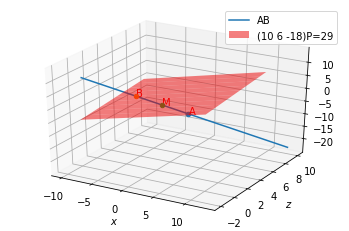
\includegraphics[width=\columnwidth]{Figure.png}
    \caption{Plot of the plane}
    \label{fig}
\end{figure}    
\end{document}
